\section{Merging 3D Maps and Atomic Structures: Rigid Fitting}
Once we have the predicted \iii{model} of any structural element included in our map, to fit that \iii{model} in the volume constitutes the next step in the modeling workflow. Two protocols have been included in \scipion with this purpose, \scommand{phenix - dock in map} (Appendix \ref{app:dockInMapProtocol}, \citep{Liebschner2019}) and \scommand{chimerax - rigid fit} (Appendix \ref{app:chimeraRigidFit}). The first one allows automatic fitting of \iii{models} in \iii{maps}, while the second one only does it when \iii{model} and \iii{map} are quite close, thus requiring manual fitting in advance. Although there is no a general rule to fit \iii{map} and \iii{model}, because it will depend on the particular problem and on our previous knowledge, in this tutorial we are going to use \phenix \ttt{dock in map} application first, followed by the final \ttt{Fit in Map} in \chimera \ttt{rigid fit}. Observe these two new steps in the modeling \scipion workflow in \ffigure{fig:scipion_workflow_rigidfit}.

 \begin{figure}[H]
  \centering 
  \captionsetup{width=.9\linewidth} 
  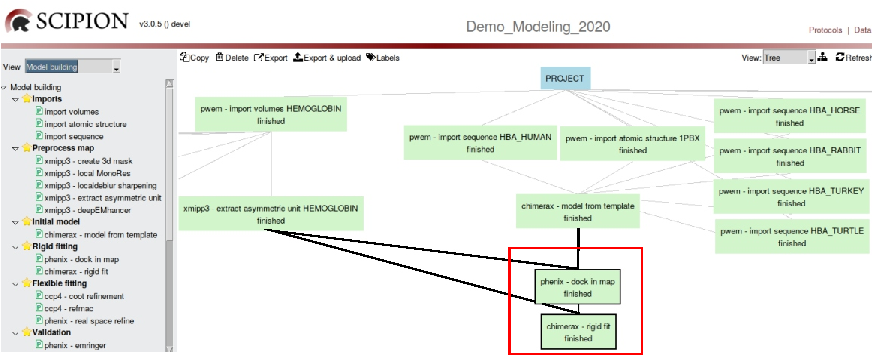
\includegraphics[width=1\textwidth]{Images/Fig67}
  \caption{\scipion framework detailing the workflow to fit the first model of the human \ttt{Hgb} $\alpha$ subunit in the map asymmetric unit.}
  \label{fig:scipion_workflow_rigidfit}
  \end{figure}

\subsection*{Initial rigid fit with \phenix \ttt{dock in map}}
 Open \scommand{phenix - dock in map} protocol (\ffigure{fig:dockInMap_protocol} (1)), and complete the form with the the extracted map asymmetric unit (2), the map resolution (3), the \iii{model} of atomic structure previously saved in \chimera (4),  and the number of copies of this atomic structure that we'd like to fit in the map, 1 in this case (5). As an additional exercise you can check the result of fitting two copies of this structure in the initial input map.
 
 \begin{figure}[H]
  \centering 
  \captionsetup{width=.9\linewidth} 
  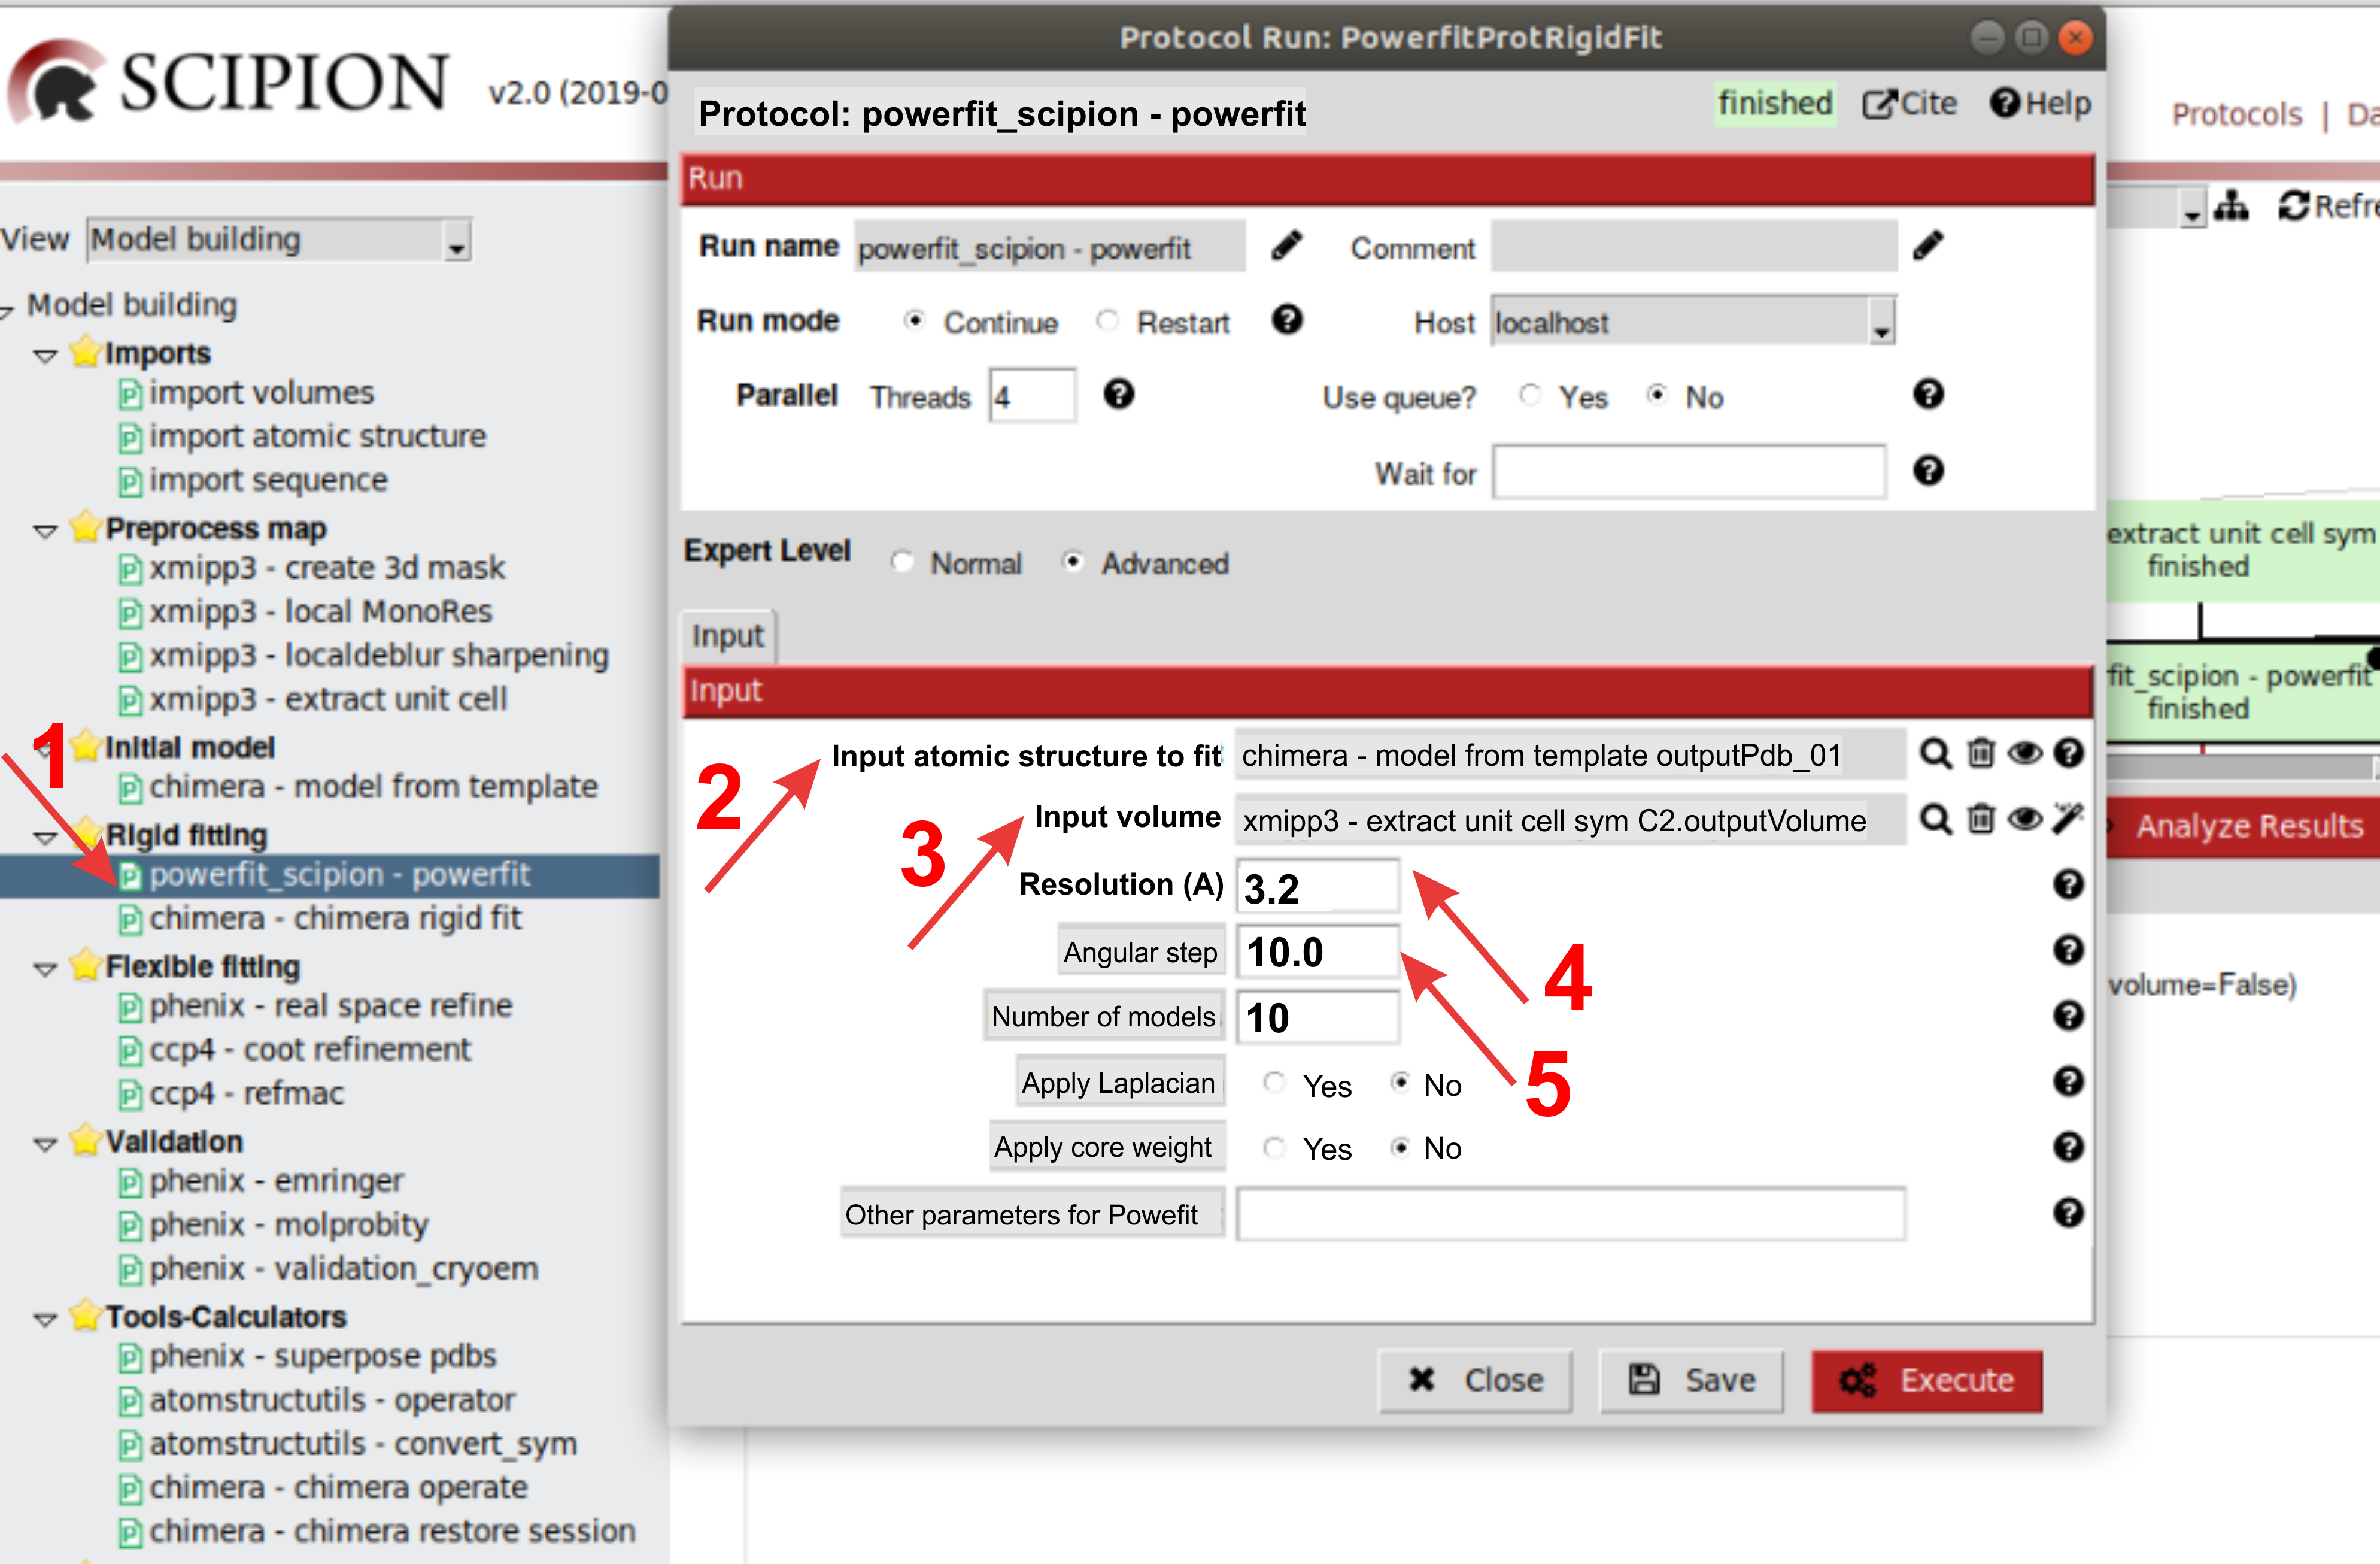
\includegraphics[width=1\textwidth]{Images/Fig18}
  \caption{Rigid fit with \scommand{phenix - dock in map} protocol: Filling in the protocol form.}
  \label{fig:dockInMap_protocol}
  \end{figure}
 
 After executing the protocol \scommand{phenix - dock in map} (\ffigure{fig:dockInMap_protocol} (6)), you can check the docking results clicking in \ttt{Analyze Results} (7). \chimera graphics window will be opened (\ffigure{fig:dockInMap_results}) showing the map and the atomic structure \iii{modeled} in its initial location (pink) and fitted in the map (green) (\ffigure{fig:dockInMap_results} (1)). 
  
 \begin{figure}[H]
  \centering 
  \captionsetup{width=.7\linewidth} 
  \includegraphics[width=0.85\textwidth]{Images/Fig20}
  \caption{Rigid fit with \scommand{phenix - dock in map}: View of docking results in \chimera.}
  \label{fig:dockInMap_results}
  \end{figure}
 
 A rough inspection of the \iii{placed\_model} in \ffigure{fig:dockInMap_results} (remark the location of the \ttt{HEME} group, for example, which should be moved slightly to the right side) shows that the fitting could be improved a little. The second protocol, \scommand{chimerax - rigid fit}, will help in this purpose.
 
 \subsection*{ Completing rigid fit with \chimera \ttt{rigid fit}}
 
 \ttt{Note before starting!!!}: As we already advised previously, we are going to use a \chimera-derived protocol (\scommand{chimerax - rigid fit}, Appendix \ref{app:chimeraRigidFit}). Remark that this use of \chimera is completely different from the use of \chimera as a visualization tool. By using the \chimera graphics window, opening it from the \scipion bottom \ttt{Analyze Results}, we can observe protocol results but we CANNOT save anything in \scipion. However, using \chimera as a tool, as it is the case in \scipion \chimera-derived protocols, we can perform different tasks, taking advantage of the available \chimera tools and, finally, we CAN save the obtained results and the working session in \scipion.\\  
 
 To complete the rigid fitting of the \iii{model} generated in the previous step, open the protocol \scommand{chimerax - rigid fit}, include again the map of the asymmetrical unit (2), and the just fitted \iii{model} of the human \ttt{metHgb} $\alpha$ subunit (3), and execute the protocol (4).
 
 \begin{figure}[H]
  \centering 
  \captionsetup{width=.9\linewidth} 
  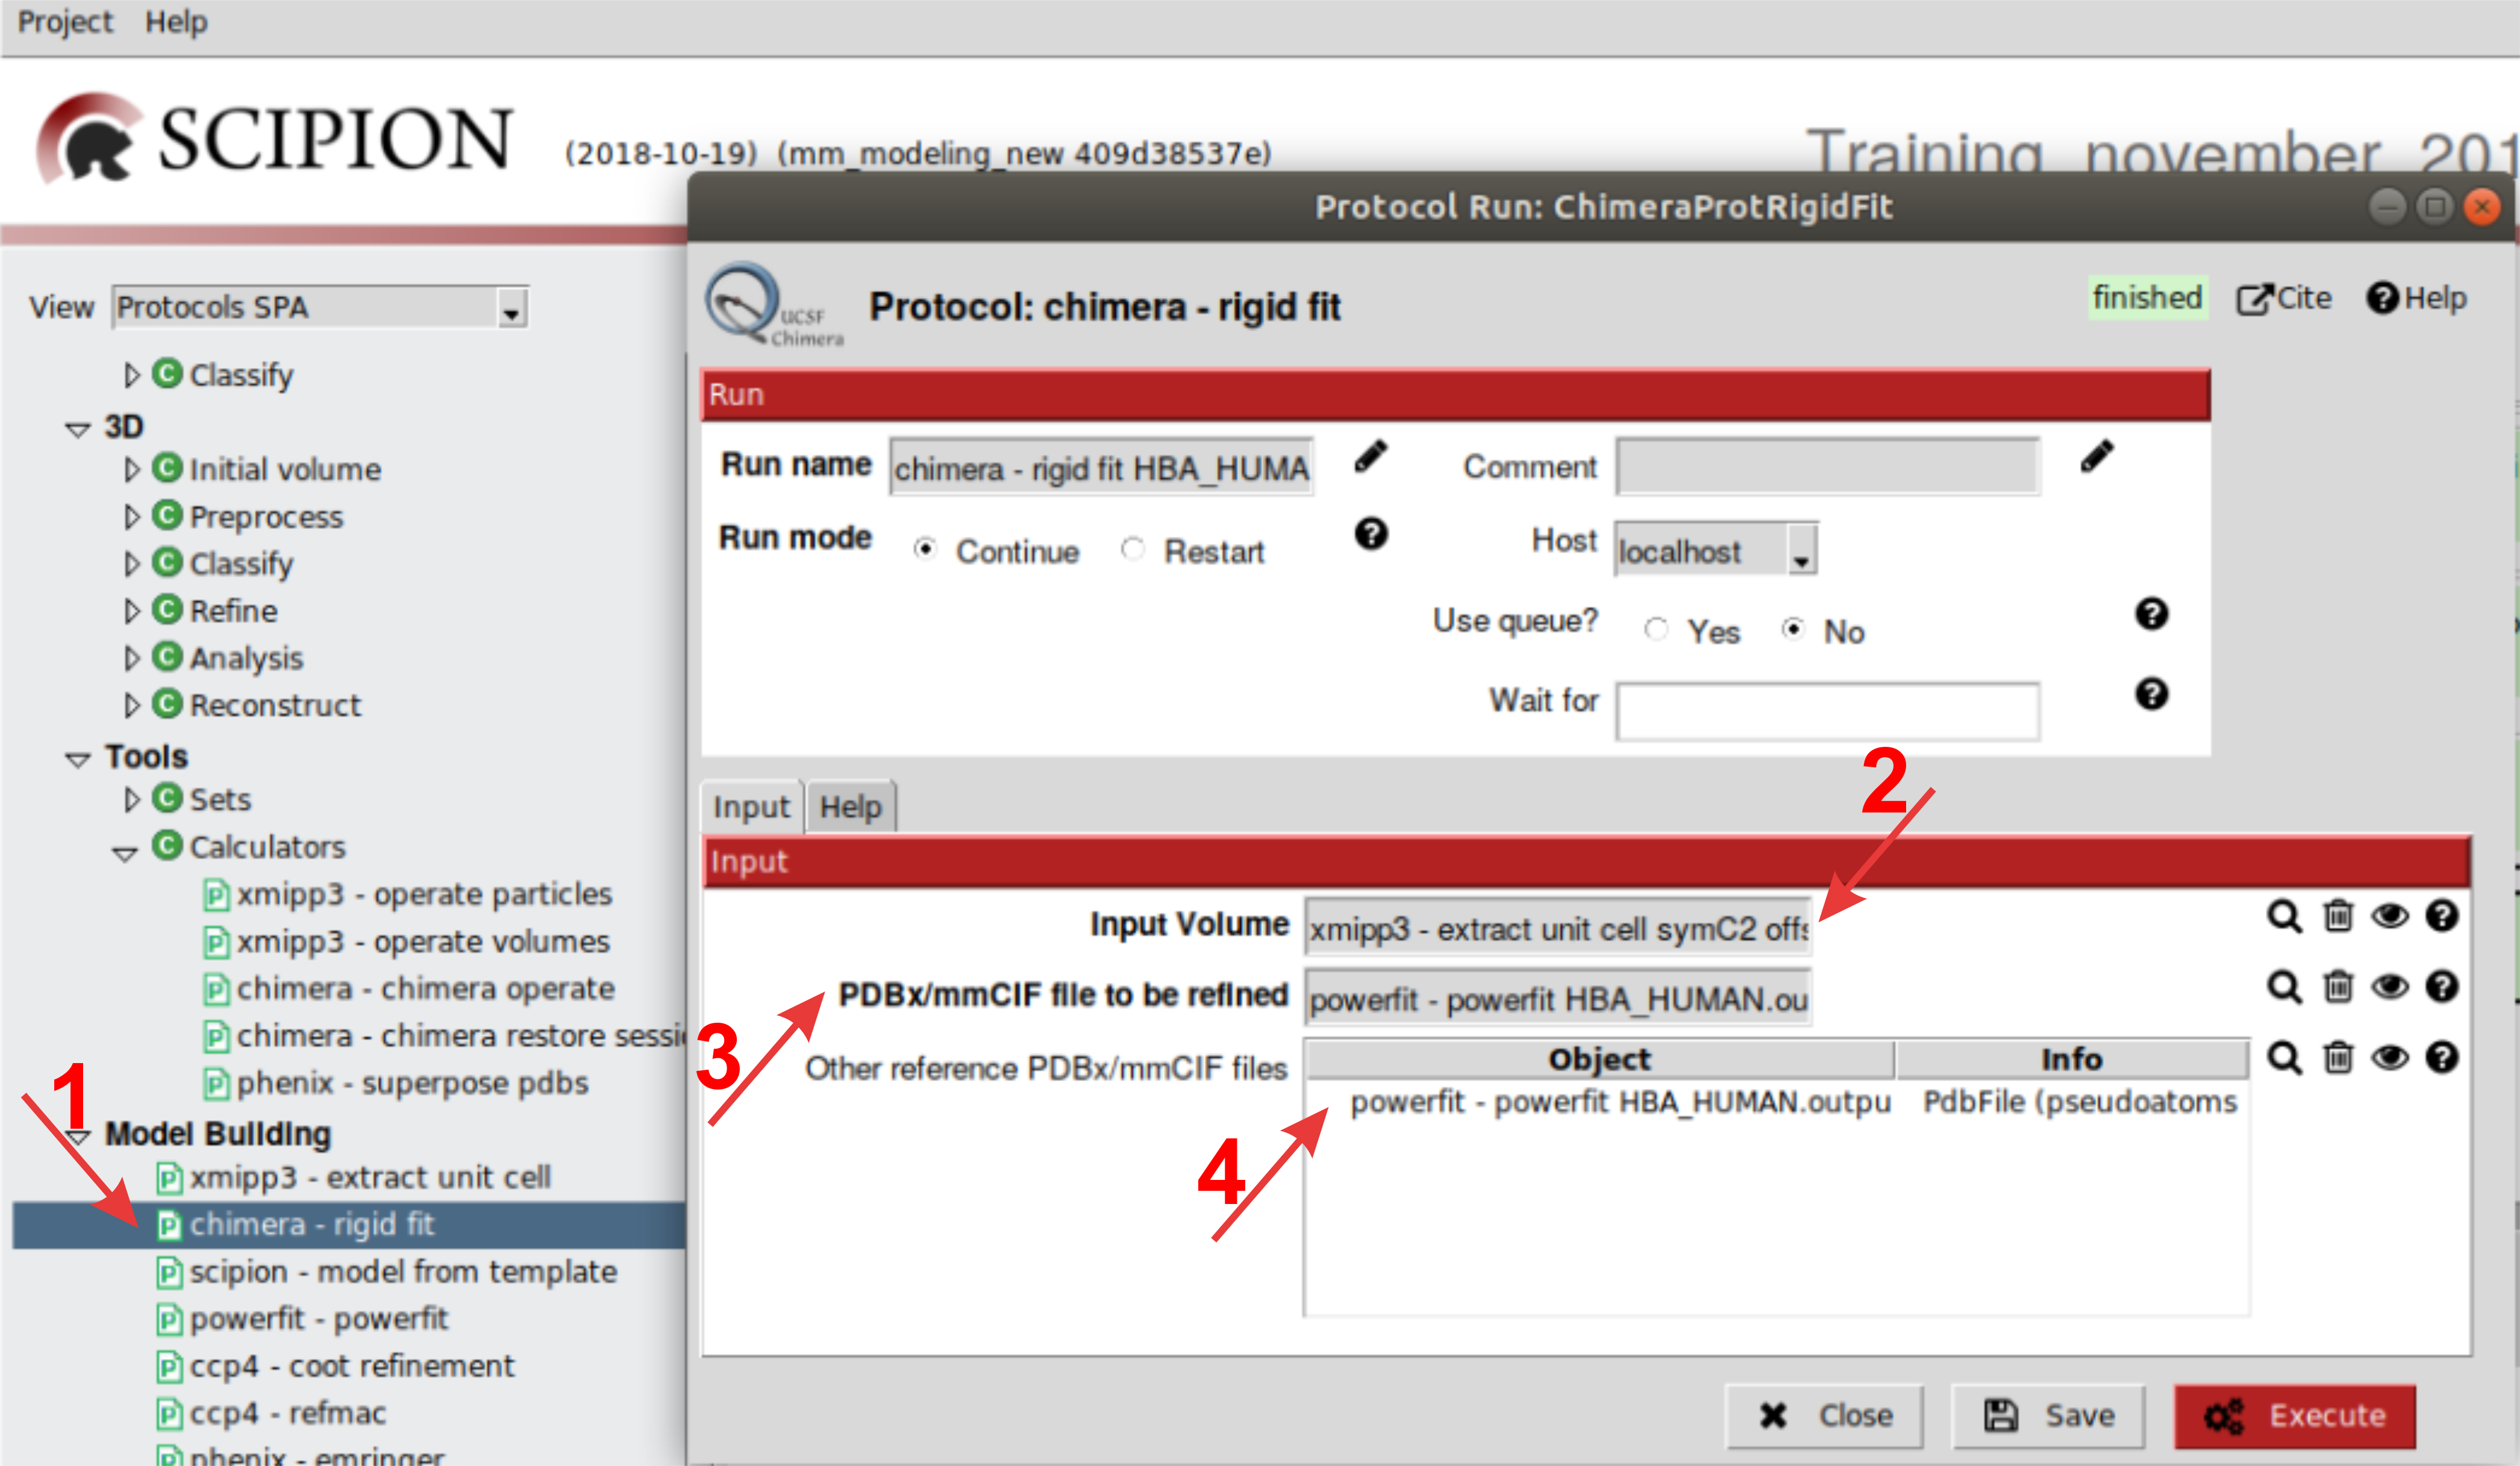
\includegraphics[width=1\textwidth]{Images/Fig21}
  \caption{Completing the \chimera rigid fit protocol form.}
  \label{fig:chimera_rigid_fit}
  \end{figure}
  
  Once opened the \chimera graphical window, we can complete the fitting of the \iii{model} to the \iii{map}, by \chimera command line or through the \chimera GUI. 
    \begin{itemize}
     \item By \chimera command line, considering that \iii{map} and \iii{model} have \iii{ID} numbers \ttt{\#2} and \ttt{\#3} (\ffigure{fig:chimera_fit_in_map} (B)):\\
            \ttt{fitmap \#3 inMap \#2}\\
    \item By the \chimera GUI: Select in the upper main menu \ttt{Tools -> Volume Data -> Fit in Map}. A small window will be opened (\ffigure{fig:chimera_fit_in_map} (A)). Select the appropriate \iii{model} to fit in the \iii{map} and press \ttt{Fit} (1) to allow the automatic rigid fitting.
    \end{itemize}

  A slight movement to the right perfectly fits \iii{map} and \iii{model}, as can be observed in (\ffigure{fig:chimera_fit_in_map} (B)). To facilitate the visual inspection of the fitting we can replace the \ttt{surface} view of the map by \ttt{mesh} as indicated in (A). Observe this time the right placement of the \ttt{HEME} group in the \iii{map} density.\\
  To use the side view as additional tool to observe the fit, select in the upper main menu \ttt{Tools -> General -> Side View}.
  
  \begin{figure}[H]
  \centering 
  \captionsetup{width=.7\linewidth} 
  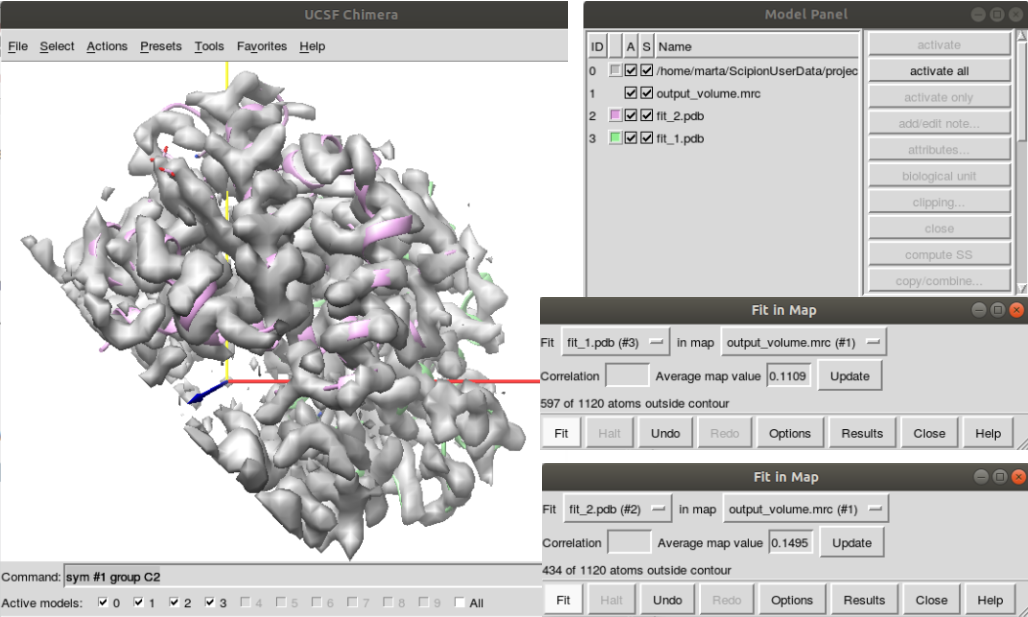
\includegraphics[width=0.85\textwidth]{Images/Fig22}
  \caption{Fit in map with \chimera.}
  \label{fig:chimera_fit_in_map}
  \end{figure}
  
  To track the \chimera fitted \iii{model} in \scipion we have to save it as fitted $model$ of the \ttt{metHgb} $\alpha$ subunit in the \chimera command line before closing the \chimera window:\\
  \ttt{scipionwrite \#3 prefix Hgb\_alpha\_}\\
  \ttt{exit}\\
  
  The string that we have included as \ttt{prefix} in the command line will allow us to follow the atomic structure in a more simple manner. In particular, if you click \ttt{Analyze Results} (\ffigure{fig:chimera_rigid_fit} (6)) the \chimera graphics window will open again and you can check the \ttt{prefix} in the the name of the saved atomic structure (\ttt{Hgb\_alpha\_Atom\_struct\_3\_003753}) in the \ttt{Models} panel of \ffigure{fig:chimera_fit_results_2} (1). Interestingly, the suffix number of the saved atomic structure (\ttt{003753}) stands for the ID protocol number and you can check it by simply surfing the mouse over the protocol (\ffigure{fig:chimera_rigid_fit} (5)).
  
  \begin{figure}[H]
  \centering 
  \captionsetup{width=.9\linewidth} 
  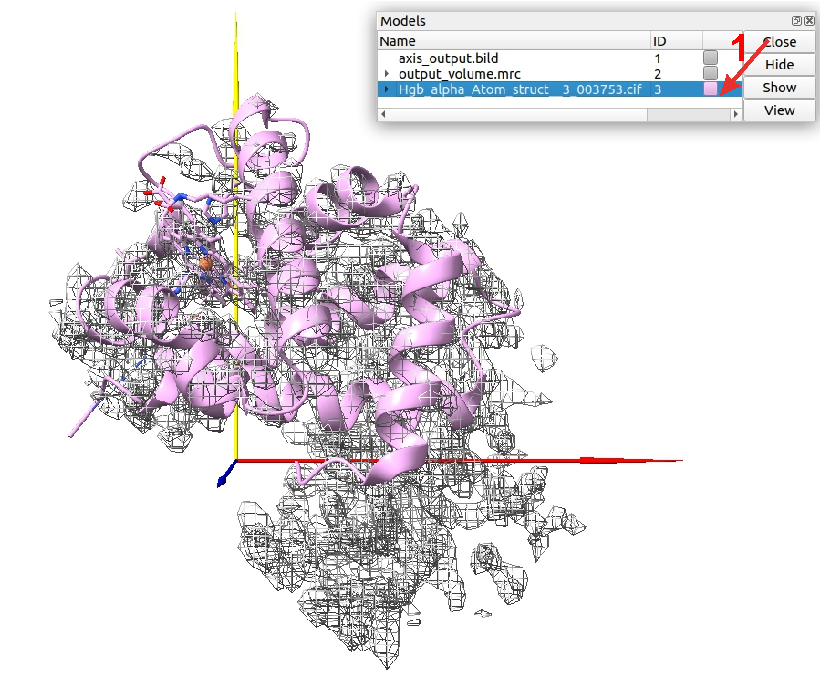
\includegraphics[width=0.85\textwidth]{Images/Fig23}
  \caption{View in \chimera graphics window of the initial \iii{model} of human \ttt{Hgb} $\alpha$ subunit fitted to the asymmetrical unit of the 3D map.}
  \label{fig:chimera_fit_results_2}
  \end{figure}

 
